\documentclass[a4paper]{article}
\usepackage[utf8]{inputenc} 
\usepackage[danish]{babel} 

\usepackage{amsmath}
\usepackage{amsfonts}
\usepackage{amssymb}
\usepackage{ulem}
\usepackage{verbatim}
\usepackage{graphicx}

\newcommand{\setR}{\mathbb{R}} 
\newcommand{\setF}{\mathbb{F}} 
\newcommand{\setN}{\mathbb{N}} 
\newcommand{\pder}[2][]{\frac{\partial#1}{\partial#2}}



\title{Week Assigment no. 50}
\author{Beate, Sarah and Freja}
\begin{document}
\maketitle

\section*{Part C}
We have chosen to make our program in the way we have because of the functionality and the design of it, makes it easier to read for the user. The plot is made into a method inside the 
\begin{verbatim}class Regression(object) \end{verbatim} 
such that we can use the method \begin{verbatim}linearAnalysis() \end{verbatim} 
to plot the data that's given.

\begin{figure}[h]
\centering
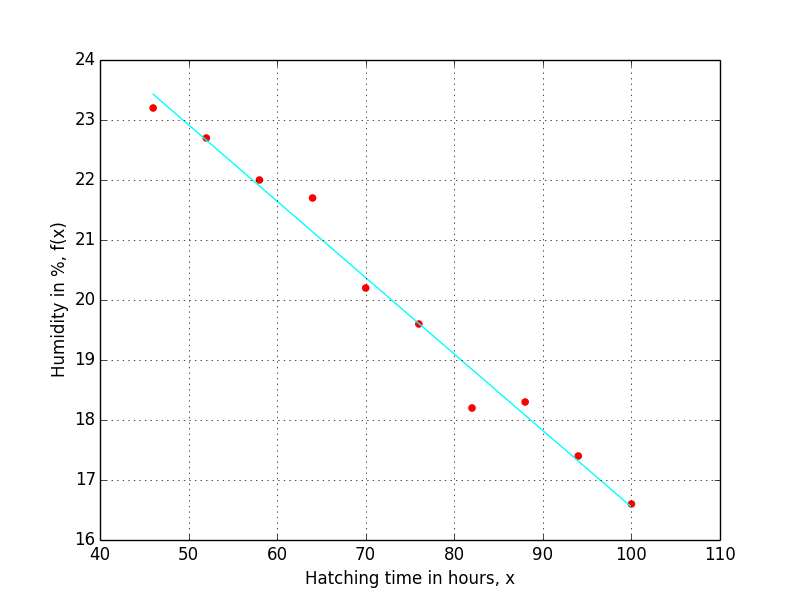
\includegraphics[width=90mm]{flueaeg}
\caption{\textit{f(x)}, min: 16.55 and max: 23.42\quad\textit{x}, min: 46.0 and max: 100.0}
\label{fig:flueaeg}
\end{figure}

\section*{Part D}
The regression line shows that a small amount of fly eggs hatch per hour. This's caused because when some of the fly eggs have hatch, there'll be in return fewer eggs left. Therefore the amount of eggs capable of hatching, will be reduced.

\section*{Part E}
We have thoroughly run our code through a series of test runs, after we ran the entire code with the original file \textit{"fluaeg.txt"}.\\
In order:
\begin{itemize}
\item no commas
\item different list lengths
\item columns with only zeros
\item the file doesn't exist 
\end{itemize}
\end{document}